%!TEX root = ../tesis.tex

\chapter{Segundo capítulo}

\section{Una sección importante}

\begin{itemize}
	\item Edad de Piedra
	\item Edad del Cobre
	\item Edad del Bronce
	\item Edad del Hierro
\end{itemize}

\begin{enumerate}
	\item Edad de Piedra
	\item Edad del Cobre
	\item Edad del Bronce
	\item Edad del Hierro
\end{enumerate}

\begin{itemize}
	\item Edad de Piedra
	\begin{enumerate}
		\item Paleolítico
		\item Mesolítico
		\item Neolítico
	\end{enumerate}
	\item Edad del Cobre
	\item Edad del Bronce
	\item Edad del Hierro
\end{itemize}
\newpage
\section{Otra sección} \label{sec:otra_seccion}

Una referencia a la \autoref{fig:plot}, dentro del \autoref{sec:otra_seccion}.

\begin{figure}[h]
	\centering
	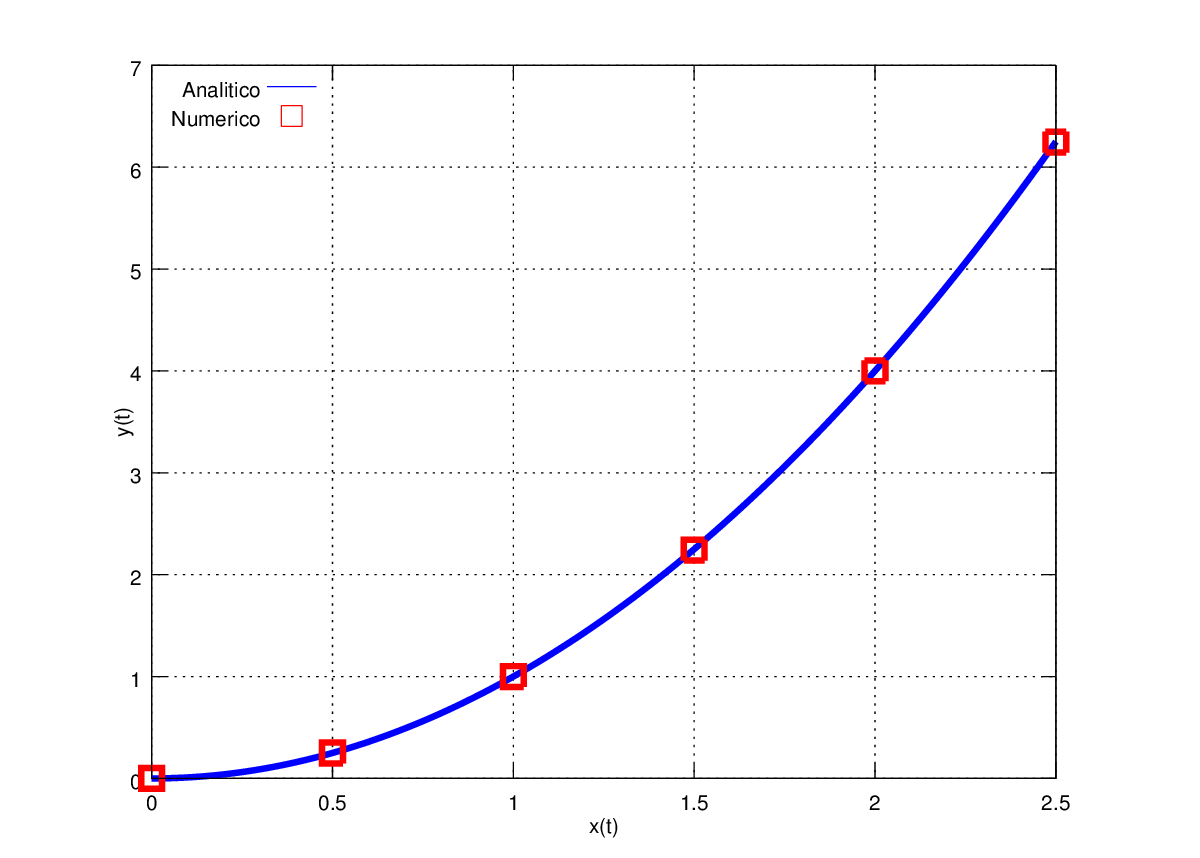
\includegraphics[width=0.7\textwidth]{Figuras/capitulo_2/x_vs_y}
	\caption{Gráfico de ejemplo.}
	\label{fig:plot}
\end{figure}

